% !TeX spellcheck = cs_CZ
%{\tikzset{external/prefix={tikz/TKY/}}
% \tikzset{external/figure name/.add={ch01_}{}}
%======================= Kapitola: Základy technické kybernetiky ===================================
\setchaptertoc
\chapter{Základy technické kybernetiky}

  \section{Vznik a vývoj kybernetiky}
    Kybernetika je jedním z nejmladších vědních oborů a její vznik spadá do čtyřicátých let 
    dvacátého století. Vznik je úzce spjat s vývojem mnoha jiných vědních oborů jako matematická 
    logika, fyziologie, neurofyziologie a s rozvojem některých technických oborů jako je 
    elektronika, výpočetní technika, řídicí technika. Kybernetika není vědou, která by pouze 
    přebírala poznatky jiných věd. Ona hledá to, co jednotlivé vědní obory spojuje, postihuje 
    určité společné rysy různých vědních oborů a má snahu o jejich integraci. 

    \begin{figure}[ht!]
      \centering
      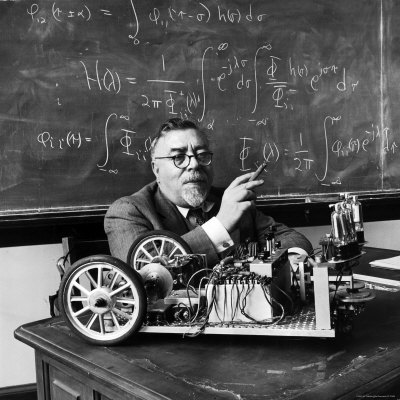
\includegraphics[width=0.8\linewidth]{Norbert_Wiener.jpg}
      \caption{Norbert Wiener (26. listopadu 1894 - 18. brezna 1964) byl americký matematik, který 
               je považován za zakladatele kybernetiky. }
      \label{tky:fig003}
    \end{figure}
  
    Historicky poskytlo impuls ke vzniku kybernetiky řešení problému řízeni palby protiletadlového 
    dělostřelectva za 2. světové války. Na tomto úkolu pracoval také americký matematik 
    \emph{Norbert Wiener}. Výsledkem matematického i konstrukčního úsilí bylo, že mířič - člověk 
    byl nahrazen přístrojem - zaměřovačem, který snímal údaje o současné poloze letadla, z ní 
    vypočítával polohu v budoucích okamžicích a servomechanismem se přenášela informace od 
    zaměřovače a počítače na kanóny. Norbert Wiener pak jako první zpracoval teorii 
    automatizovaných systémů řízeni pro účely protiletecké obrany. Tuto teorii zobecnil pro všechny 
    druhy technických, biologických a společenských systémů. Shrnul ji ve své proslulé knize 
    \emph{Kybernetika neboli řízení a sdělování v živých organismech a strojích}. Tato kniha vyšla 
    v roce \num{1948} a stala se světovým vědeckým bestsellerem. Svého autora proslavila jako 
    zakladatele kybernetiky.
    
    Řešení praktických (a bohužel vojenských) problémů použití elektronických počítačů k řízení 
    střel inspirovalo Wienera ke studiu řízení se zpětnou vazbou. Spolu s neurofyziologem 
    \emph{Arturem Rosenbluethem} hledali analogie k technickým zpětnovazebním systémům pro navádění 
    střel na pohyblivý cil. Takovou analogii nalezli u některých biologických systémů - konkrétně v 
    nervové soustavě živých organismů. Myšlenka zpětné vazby u živých a neživých systémů se stala 
    základem kybernetické koncepce vyložené v citované knize. Hledáni analogií mezi živým 
    organismem a strojem (případně také společnosti) znamená postihnout společné znaky zdánlivě 
    naprosto různorodých systémů. A tyto analogie pak vedou k používáni matematického a logického 
    aparátu i tam, kde to dosud nebylo možné.
    
    Nemůžeme ovšem nevidět všechny předcházející tendence a faktory v historii společnosti, které 
    vedly ke vzniku kybernetiky. Bylo by nesprávné tvrdit, že pouze Norbert Wiener a několik jeho 
    spolupracovníků vytvořilo kybernetiku. Její vznik byl pokračováním určité tendence, která se 
    projevovala již dávno předtím. Kybernetiku musíme chápat jako výsledek rozvoje materiálních sil 
    lidské společnosti a rozvoje vědeckého poznáváni světa.
    
    Název kybernetika pochází z řeckého slova \uv{kybernétés} neboli \uv{kormidelník}, \uv{člověk 
    řídící loď}. Objevuje se v dílech řeckých filosofů, např. v Platonově díle Dialogy; zde se 
    tímto termínem vyjadřuje \uv{umění řídit lodě a administrativně spravovat provincie}. V 
    novověku použil termín kybernetika A. M. Ampére v encyklopedii a to ve smyslu \uv{vědy o řízení 
    společnosti}. Termín se neujal a tak to byl až Wiener, který jím nazval nově vznikající vědní 
    obor. \cite[s.~6]{Svarc1986}.

    \subsection{Základní pojmy kybernetiky a její vymezení}
      Pro kybernetiku jsou charakteristická tři základní hlediska, z kterých nazírá na problémy a z 
      kterých dané problémy řeší. Jsou to

      \luagraphic[0.8]{tky_fig004.pdf}{Základní hlediska kybernetiky}{tky:fig004}
      
      
      Tím se dostáváme k nejzákladnějších pojmů kybernetiky: \textbf{systém}. \textbf{informace} a 
      \textbf{řízení}, Z těchto hledisek se pak vyvinuly základní obory teoretické kybernetiky - 
      teorie systémů, teorie informace a \hyperlink{tky:regulace}{teorie řízení}.
      
      Jako příklad vysvětlující tato hlediska kybernetiky si zvolme automobil. Automobil je z 
      hlediska konstruktéra složité technické zařízení, sloužící k dopravě osob a nákladu, které je 
      vyrobeno z různých materiálů. Je sestaven z mnoha součásti, pohon je motorem spalovacím nebo 
      vznětovým, k provozu jsou nezbytné látky jako benzín, oleje, voda, ... .To vše je důležité a 
      podstatné z hlediska konstruktéra automobilu, ale ne z hlediska kybernetiky.

      \luagraphic[0.8]{tky_fig001.pdf}{ }{tky:fig001}

      Jaká jsou tedy hlediska kybernetiky? Kybernetika vidí v automobilu především tzv. 
      \textbf{dynamický systém}, jehož činnost je spojena s člověkem - řidičem a je ve vztahu k 
      okolnímu světu. Automobil uvažovaný jako systém se skládá ze dvou podsystémů (subsystémů). 
      Prvním z nich je vlastní vozidlo, druhým je člověk. Každý podsystém se pak skládá z 
      elementárních jednotek, vzájemně propojených, tzv. \emph{prvků systému}. Mezi prvky systému 
      existují různé vztahy. Ale nejenom mezi prvky nebo podsystémy existuji vztahy.

      Automobil není izolovaným systémem a proto má také četné vztahy k okolí. K okolí \uv{systému 
      automobil} patří ty části okolního světa, které mají vliv na jeho činnost. Jsou to např. 
      vozovka, křižovatky, zatáčky, jiná vozidla, chodci, dopravní značky apod. Na všechny vlivy 
      okolí reaguje systém automobil určitým způsobem. Reakce systému na okolí se nazývá 
      \textbf{chováni systému}. Pokud sleduje kybernetika automobil tímto způsobem, jedná se o 
      \emph{systémové hledisko} kybernetiky  (obr. \ref{tky:fig001}). Předběžně si vymezme pojem 
      systém jako soubor prvků, mezi nimiž existuji nějaké funkční vztahy. Sledujeme-li vzájemné 
      působeni systému a jeho okolí, jde o druhé základní kybernetické hledisko. Poněvadž se toto 
      působeni realizuje výměnou informaci mezi systémem a okolím, mluvíme o \emph{informačním 
      hledisku}. Pod pojmem informace si představíme zprávu, která má pro některé ze zúčastněných 
      systémů určitý význam. Nositelem informace jsou tzv. \textbf{signály}.
      
      Doposud jsme uvažovali prostou výměnu informaci mezi dvěma systémy. Je-li ale informace 
      využívána přijímacím systémem pro další činnost, pro dosaženi určitého předem stanoveného 
      cíle, pak už se jedná o \emph{řízení}. Pojem řízení vymezíme jako \emph{proces výměny 
      informace mezi dvěma systémy}, který se uskutečňuje plánovitě pro dosažení určitého cíle. Při 
      řízení se uplatňuje informační působení řídicího systému na řízený systém. Tím se dostáváme k 
      třetímu kybernetickému hledisku a to je \emph{hledisko řízení}. Zdůrazněme, že toto hledisko 
      provádí pouze informační bilancování a nikoliv látkové nebo energetické.
      
      Vraťme se k našemu automobilu. Systém automobil má dva podsystémy vozidlo a řidiče. Mezi nimi 
      probíhá informační výměna, jejíž cílem je pohyb automobilu po stanovené dráze, např. v přímém 
      směru. Řidič reaguje na nerovnosti vozovky nebo na boční vítr, které vychyluji vozidlo z 
      přímého směru tím, že pootáčí volantem. Řidič je tedy řídícím systémem a vozidlo řízeným 
      systémem a výměna informací probíhá za účelem udrženi pohybu vozidla v přímém směru - jedná 
      se o \textbf{proces řízení}.
      
      Všimněme si momentu, že řidič otáčí volantem na základě toho, jaký účinek vyvolalo předchozí 
      pootočení. Neustále sleduje směr vozidla a vyrovnává odchylky od přímého daného směru. Takový 
      způsob řízení označujeme v kybernetice jako \textbf{řízení se zpětnou vazbou} neboli 
      \textbf{regulace}. Systémy se zpětnou vazbou se tedy nazývají \textbf{regulační systémy}. 
      Systém automobil (řidič + vozidlo) můžeme pokládat za regulační systém, který je regulován na 
      přímý směr jízdy.
      
      Poněvadž systémy řízení se zpětnou vazbou, tedy regulační systémy, jsou pro kybernetiku 
      charakteristické, nazýváme třetí kybernetické hledisko také \emph{hlediskem regulačním}. 
      Samozřejmě existuje rovněž \textbf{řízení bez zpětné vazby}; v tom případě se mluví jen o 
      \textbf{systémech řízení} nebo o \textbf{systémech ovládání}.
      
      Řízení jako vzájemná interakce mezi systémy nebo mezi systémem a okolím probíhá vždy v 
      určitém pořadí činnosti některého ze systémů. obvykle řídicího. Soubor pravidel, podle něhož 
      řídící systém vykonává sled činností za účelem řízení, se nazývá \textbf{algoritmus}. Obecně 
      je \emph{algoritmus soubor pravidel, podle něhož probíhá řízení}.
      
      U zvoleného příkladu s automobilem bychom mohli například sestavit algoritmus spouštění 
      motoru, algoritmus vyjíždění automobilu, algoritmus předjíždění, atd. Algoritmy jsou objektem 
      zkoumání jednoho z oborů teoretické kybernetiky - \emph{teorie algoritmů}.
      
      Pe předběžném objasnění základních hledisek kybernetiky a základních pojmů kybernetiky je 
      možné se pokusit vyložit, ce vlastně kybernetika je a čím se zabývá. Jednotlivý autoři, kteří 
      se pokoušejí podat definici kybernetiky, protěžují více nebo méně některé ze tří základních 
      kybernetických hledisek (hledisko systémové, hledisko informační, hledisko řízení). Většina 
      starších definic kybernetiky vychází z klasické definice jejího uznávaného zakladatele 
      Norberta Wienera, který ji definoval jako \uv{vědu o řízení a sdělování v živých organismech 
      a strojích}. Tato definice, která je nerozlučně spjata s jejím vznikem, protěžuje hledisko 
      informační a hledisko řízení. Jejím nedostatkem je, že ještě nedoceňuje systémový přístup, 
      systémové hledisko při řešení problémů. Dále jako objekty zkoumání (tedy systémy) zahrnuje 
      pouze živé organismy a stroje. Nezahrnuje tedy další důležité objekty zkoumané dnešní 
      kybernetikou jako jsou objekty společenské a ekonomické a neuvažuje systémy matematické, 
      lingvistické a další a z technických systémů dnes tak různorodých se omezuje jen na stroje. 
      Ani informační hledisko této definice není úplné, protože se omezuje pouze na přenos 
      informaci a neuvažuje dnes tak důležité procesy uchování a zpracováni informace.
      
      Podobnými nedostatky se vyznačovaly definice kybernetiky dalších autorů. Byl to vždy 
      jednostranný přístup a neúplnost jednotlivých hledisek. Proto nelze žádnou z definic 
      akceptovat s definitivní platností.
      
      Nebudeme se tedy snažit za každou cenu zformulovat vyčerpávající definici, ale uveďme si 
      charakteristické rysy kybernetiky jako vědy.
      
      Kybernetika se zabývá různými rozdílnými problémy, které však byly většinou známy a zkoumány 
      před vznikem kybernetiky, např. krevní oběh, podmíněný reflex, radiolokace, konstrukce 
      počítačů, řízení různých technických zařízení, kódování atd. Kybernetika vnáší do těchto 
      problémů nový pohled, neboť si všímá toho, že na určitém stupni organizace a vývoje systémů 
      vzniká nový proces řízení. Tento proces se projevuje výměnou informací v systémech, kterým se 
      chování systémů zaměřuje k určitému cíli.
      
    \subsection{Rozdělení kybernetiky}
      Z praktického hlediska můžeme kybernetiku rozdělit podle přístupu a aplikací:
      \begin{itemize}[noitemsep]
        \item \textbf{teoretická kybernetika},
        \item \textbf{aplikovaná kybernetika}.
      \end{itemize}

      \emph{Teoretická kybernetika} studuje především obecné vlastnosti a chování systémů. Zabývá 
      se obecným popisem vlastností a chování systémů. Z tohoto pohledu zahrnuje teoretická 
      kybernetika \emph{teorii systémů} a \emph{teoretickou informatiku}.
      
      \emph{Aplikovaná kybernetika} představuje použití kybernetického přístupu při analýze, 
      modelování a simulaci a návrhu systémů, dále aplikuje poznatky kybernetiky do dalších 
      oblastí. Aplikovaná kybernetika zasahuje do mnohých oblastí lidské činnosti - zahrnuje totiž 
      mj. následující obory:
      
      \begin{itemize}\addtolength{\itemsep}{-0.1\baselineskip}
        \item \textbf{Teoretická kybernetika}
              \begin{itemize}\addtolength{\itemsep}{-0.1\baselineskip}
                \item \emph{Dynamické systémy}: zpětná vazba, stavový popis, stochastické systémy,
                      řízení, aj.
                \item \emph{Přenos informace}: informační entropie, kapacita komunikačního kanálu, 
                      aj. 
                \item \emph{Umělá inteligence}: strojové vnímání a učení, multi-agentní systémy, 
                      robotika, modelování neuronových sítí, konekcionismus, vazba člověk-stroj, ...
                \item \emph{Teorie rozhodování}, her, teorie složitosti, chaotické systémy, aj.
              \end{itemize}
        \item \textbf{Informatika}
        \item \textbf{Biokybernetika}
        \item \textbf{...}
      \end{itemize}
      
  \section{Teorie systémů}
     Teorie systémů je jedna ze základních disciplin teoretické kybernetiky. Na druhé straně je ale 
     teorie systémů součásti tzv. \emph{obecné teorie systémů}, jejíž principy rozpracoval americký 
     biolog Ludwig von Bertalanffy. Pokusme se o vymezení vztahu mezi kybernetikou a teorií systémů.
     \cite[s.~11]{Svarc1986}.
     
     Obecná teorie systémů studuje systémy libovolné povahy, přičemž se zajímá o charakter prvků 
     systému, charakter vazeb mezi prvky a chováni systému. Důležitým pojmem je zde \textbf{vazba 
     mezi prvky} a pojem \textbf{chování systémů}. Zatímco obecná teorie systémů se zajímá o 
     libovolný druh vazeb mezi prvky a libovolné chování systémů, kybernetiku zajímá specifický 
     druh vazeb a specifické chování. Kybernetika studuje pouze ty vazby, které jsou realizovány 
     přenosem informace a chování, které lze zahrnout pod \textbf{pojmem řízení}. A to je náplni 
     teorie systémů jako discipliny teoretické kybernetiky.
     
     \textbf{Přenos informace} a \textbf{řízení} nejsou od sebe \emph{oddělitelné}. Aspoň tak, že 
     není možné řízení bez přenosu informace. Je však už sporné, je-li každý přenos informace již 
     řízením. Můžeme říci, že systémy mezi nimiž probíhá proces řízení musí mít určitou specifickou 
     strukturu a musí být mezi nimi zajištěn přenos informace. Pokud existuje pouhá výměna 
     informací mezi systémy, mluvíme o \textbf{informačních systémech}.
     
     \emph{Obecnou teorii systémů} tedy \emph{nemůžeme} zahrnout do kybernetiky; s kybernetikou má 
     společnou jen určitou část, která je zaměřena na studium systémů z hlediska informačních 
     vazeb. Hlavním úkolem obecné teorie systémů je postihnout a vyjádřit exaktním způsobem 
     vlastnosti a vztahy ve složité a dynamické (v čase se měnící) \emph{objektivní realitě} tak, 
     aby se neztratila její komplikovaná struktura a složitost. Jestliže dříve byl nějaký přírodní 
     nebo společenský jev pokládán za vysvětlený, když se nalezla jeho příčina, pak při systémovém 
     přístupu musí bý nalezena struktura a dynamika každého objektu, který se na daném jevu podílí.
     
     \subsection{Charakteristika základních pojmů z teorie systémů}
       Pro práci se složitými a rozsáhlými objekty, jako jsou například řízení výrobních a
       technologických procesů, je nutný \textbf{systémový přístup}. Například technologický proces
       exploatace uhlí na hlubinných nebo povrchových dolech, je charakterizován různorodostí
       pracovních činností, na něž působí celá řada vlivů. Komplexně jde o mnoha rozměrný
       dynamický celek, který se neustále mění v čase a v prostoru.
       
       \emph{Systémový přístup spočívá v tom, že jevy vyskytující se při řešení vzniklých problémů, 
       jsou chápany komplexně, se všemi souvislostmi ve svém dynamickém vývoji.}
       
       V souvislosti se systémovým přístupem je nejdůležitějším pojmem \textbf{systém}. Jestliže 
       chceme v dalším uvést základní pojmy teorie systémů, musíme nejdříve tento pojem vysvětlit. 
       Předběžně jsme ho vymezili jako \emph{soubor prvků, mezi nimiž existuji nějaké funkční 
       vztahy a který má jako celek vztah ke svému okolí}. Jinými slovy: \emph{Stanovíme- li 
       vztahy, mezi na sebe navzájem působících objektů materiální, ale i nemateriální povahy, je na
       objektivní realitě vytvořen systém.} Jiní autoři podávají tyto definice:
       \begin{itemize}[noitemsep]
         \item Bertalanffy (1956): Systém je komplex prvků nacházejících se ve vzájemné interakci.
         \item Hall - Fagen (1966): Systém je souhrn prvků spolu se vztahy mezi prvky a mezi jejich 
               vlastnostmi.
       \end{itemize}

       \begin{definition}
        \textbf{Systém} je definován jako účelově uspořádaná množina prvků a množina vazeb mezi 
        nimi, s dynamickým chováním, které společně určují vlastnosti celku.
        \begin{equation}
          \mathscr{S} = \{S,R \},
        \end{equation}
        kde
        \begin{description}[leftmargin=5em,style=nextline]
          \item[\hspace{2em}\(S \ldots\)] \emph{množina všech prvků},
          \item[\hspace{2em}\(R \ldots\)] \emph{množina relací mezi prvky, reprezentující vzájmené 
                                         funkční vztahy jednotlivých prvků a vztah systému k okolí.}
        \end{description}
       \end{definition}
       
       V rámci dekompozice systému lze vyčlenit \textbf{podsystém}. Podsystém je podmnožina
       systémových prvků a vazeb, která je z nějakého důvodu vyčleněna ze systému a je chápána
       jako nový systém nebo jako prvek.
       
       \begin{definition}
        \textbf{Prvek} je část systému, který tvoří na dané rozlišovací úrovni dále nedělitelný 
        celek, jehož strukturu nechceme, nebo již nemůžeme v rámci analýzy rozlišit.
       \end{definition}
       
       \begin{note}
         \textbf{Rozlišovací úrovní} se označuje stupeň podrobnosti zkoumání systému. Změnou        
         rozlišovací úrovně se může dřívější prvek systému stát podsystémem, popřípadě i systémem a 
         naopak. Dekompozicí systému na jednodušší prvky, se zvyšuje rozlišovací úroveň.
       \end{note}
       
     \subsection{Klasifikace systémů}
       Někdy rozlišujeme pojem \textbf{statický} a \textbf{dynamický systém}, ale spíš známe pouze 
       systémy dynamické. Statický systém je totiž v čase konstantní, neměnný. Mezi statické 
       systémy můžeme někdy zařadit i systémy, u nichž se vlastnosti prvků mění velmi pomalu. V 
       přírodě se statické systémy prakticky nevyskytují, spíše se jedná o systémy s pomalou změnou 
       vlastností na čase. Naproti tomu dynamický systém je takový systém, u kterého existuje 
       alespoň jedna proměnná závislá na čase. Většina systémů je dynamických. V dalším textu jsou 
       proto popsány především \textbf{dynamické systémy a řídicí (regulační) systémy se zpětnou 
       vazbou}.
       
       Dynamické vlastnosti lineárních systémů lze popsat lineárními diferenciálními rovnicemi s 
       konstantními koeficienty a operátorovými přenosy. Dynamické vlastnosti nelineárních systémů 
       lze popsat nelineárními diferenciálními rovnicemi.
       
       Existují dvě možnosti studia dynamického systému. Prvním způsobem je zkoumání \emph{vnitřní 
       struktury systému}, tzn. vnitřní závislosti prvků a dále nás zajímají, jaké vnitřní změny 
       vznikají v systému při působení vnějších vlivů. To je podstatou \textbf{vnitřního popisu 
       dynamického systému}.
       
       Druhým způsobem je pojímání systému jako celek a studování pouze otázky, jaké výsledné 
       reakce systému vyvolávají vnější vlivy. Tomuto druhému způsobu se budeme věnovat při 
       \textbf{vnějším popisu dynamických systémů}.
     
     
  \section{Teorie informace}
    \textbf{Informace} jako stěžejní pojem kybernetiky, je pojem značně široký a hodně diskutovaný. 
    Je používán v celé řadě definic vymezujících předmět kybernetiky jako vědy, přičemž informační 
    hledisko považují někteří autoři za nejdůležitější.
      
    Přesná definice pojmu informace neexistuje. Obecně se tento pojem používá volně, v intuitivním 
    chápaní se vztahuje k pojmům jako zpráva, údaj, poznatek apod. Z hlediska kybernetiky je toto 
    chápáni příliš zúženo, neboť kybernetika sleduje přenos informace mezi dvěma nebo více systémy 
    s tím, že cílem přenosu může být řízení chování některého ze systému. Kybernetika říká, že 
    informace je jakékoliv sdělení, kterého lze reálně (právě nyní) nebe potenciálně (v budoucnu 
    při vhodné příležitosti) použit k řízeni systému.
    
    Pojem informace je \emph{pojmem abstraktním} a jako takový má \emph{nehmotnou povahy}. 
    Současně však informace má smysl jen ve spojení s hmotou a to jak z hlediska přenosu, tak z 
    hlediska obsahu (i abstraktní představy jsou spjaty s existenci hmoty).
    
    Informace (sděleni) má
    \begin{itemize}\addtolength{\itemsep}{-0.4\baselineskip}
      \item \textbf{formu},
      \item \textbf{obsah},
      \item \textbf{význam}.
    \end{itemize}
    \textbf{Forma} informace neboli sdělení musí být přístupná systémům, mezi nimiž dochází k 
    výměně informaci a je důležitá pro proces přenosu informace. Pro proces řízení systémů je 
    podstatný \textbf{obsah a význam informace} (sdělení). \textbf{Sdělení} je \emph{informační, 
    sémantický a pragmatický obsah}. \textbf{Informační obsah} vyjadřuje kvantitativní míru 
    informace v dále definované jednotce \textbf{bit}. Používáme pro něj termín míra či množství 
    informace. \textbf{Sémantický obsah} vyjadřuje významovou stránku znaků při jazykové komunikaci 
    a nedá se měřit (\emph{sémantika} - nauka o významu slov). \textbf{Pragmatický obsah} určuje 
    významnost sdělení a prioritu jednotlivých zpráv pro příjemce.
    
    Každá forma hmoty, která nese informaci se nazývá \textbf{zpráva}. Zpráva je hmotným nositelem 
    informace. Zpráva je způsob vyjádření informace textem, obrazem, řečí, posloupností znaků atd. 
    Zpráva může být tedy např. číslo (posloupnost číslic), abecední text (posloupnost písmen), 
    spouštěcí signál (posloupnost napěťových úrovní). Pojmy informace a zpráva nelze zaměňovat. 
    Informace jo pojem abstraktní, zpráva jo konkrétní materiální formou informace, bez níž by 
    informace neměla smysl a nemohla by být přenášena a působit na systémy, kterým je určena. Pojem 
    zpráva bývá někdy nahrazován užším pojmem \textbf{signál}. Signál je fyzikální realizace zprávy 
    ve formě elektrického proudu resp. elektromagnetických vln.
      
    Sledujeme-li blíže jakoukoliv dostatečně dlouhou zprávu, pak zjistíme, že je vždy vytvářena z 
    posloupnosti nějakých základních elementů - \textbf{prvků}. Možný počet odlišných prvků, ze 
    kterých je taková zpráva vytvářena, může být bud \emph{konečný} nebo \emph{nekonečný}. Tak 
    např. psaná zpráva ve formě českého textu je posloupností různých kombinací písmen české 
    abecedy. Možný počet různých písmen - prvků je konečný a je dán počtem písmen české abecedy.
      
    Základní prvky, ze kterých je vytvářena zpráva, bývají obecně nazývány \textbf{písmena} a celý 
    \emph{soubor} všech \emph{možných prvků} bývá nazýván \textbf{abecedou zdroje}. Zpráva je pak 
    vytvářena výběrem prvků z abecedy zdroje a jejich sestavou v posloupnost prvků. Přitom 
    libovolný prvek abecedy se může ve zprávě libovolně opakovat. Abychom mohli odlišovat prvky 
    abecedy od prvků, z nichž je sestavena konkrétní realizace zprávy, budeme libovolný prvek 
    realizace zprávy nazývat \textbf{symbol}. Nechť má abeceda zdroje celkem \(s\) možných různých 
    prvků. Nechť je délka zprávy, tj. počet symbolů, z nichž je složena realizace zprávy, dána 
    počtem \(L\) symbolů. Celkový možný počet \(L\) různých realizaci zpráv délky \(n\), které 
    mohou být produkovány zdrojem s abecedou o \(s\) prvcích a které se budou lišit nejméně v 
    jednom symbolu, je
    \begin{equation}\label{tky:eq0001}
      L = s^n
    \end{equation}
    (počet všech možných \emph{variací n symbolů s opakováním}, které lze vytvořit z \(s\) prvků).
    
    Má-li abeceda zdroje \emph{konečný počet} \(s\) možných prvků, pak takový zdroj nazýváme 
    zdrojem \textbf{diskrétních zpráv} (diskrétní zdroj). Má-li abeceda zdroje \emph{nekonečný 
    počet prvků}, pak ho nazýváme zdrojem \textbf{spojitých zpráv} (spojitý zdroj).
    
    \begin{example}
      Kolik zpráv o délce \num{10} symbolů můžeme vytvořit z abecedy o \num{2} písmenech?
      \newline
      Řešení: Počet realizaci \(L\) zpráv je dán vztahem (\ref{tky:eq0001})
      \begin{equation*}
        L = s^n = 2^{10} = 1024
      \end{equation*}      
    \end{example}
      
    \subsection{Přenos zpráv}
      Zprávu lze přenést buď \emph{přímo}, přenesením nosného média (pergamen, magnetická páska, 
      optický disk), anebo \emph{nepřímým} způsobem prostřednictvím \emph{signálu}, který je 
      realizací zprávy ve formě změn některé fyzikální veličiny, nejčastěji elektrického proudu.
      
      Při nepřímém způsobu \textbf{zdroj informace} generuje prostřednictvím \textbf{kodéru} 
      (kódovacího zařízeni) signály, které se přenáší \textbf{kanálem}. Kanál je vlastně cesta, 
      která přenáší změny dané fyzikální veličiny, aby mohla být zpráva přenesena z jednoho místa 
      na druhé. Je tvořený prostředím, kterým se přenáší signál. Může to být např. telefonní 
      vedeni, trubka pro přenos tlakového signálu, akustické nebe elektromagnetické vlnění.
      
      Na výstupu kanálu je signál přijímán \textbf{příjemcem informace} (Člověk nebe zařízeni). 
      Zná-li příjemce zákon, podle kterého byla provedena transformace zprávy na vstupu kanálu, pak 
      může určit zprávu obsaženou v přijatém signálu. To provede tzv. \emph{dekódováním} v zařízeni 
      zvaném \textbf{dekodér}. Souhrn všech uvedených objektů vytváří \textbf{sdělovací soustavu}.

      \begin{figure}[ht!]
        \centering
        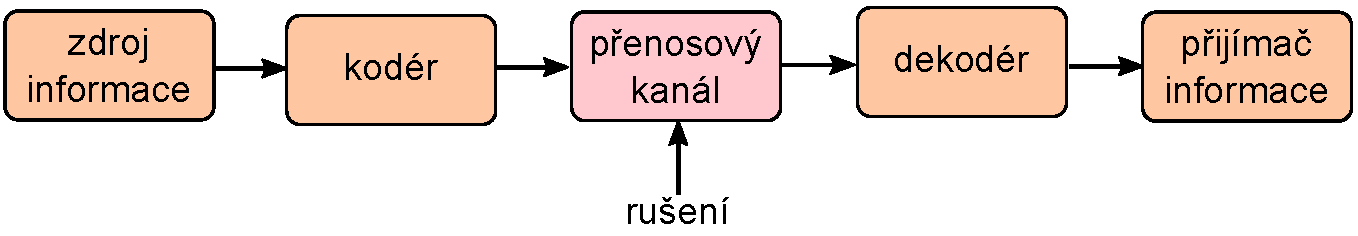
\includegraphics[width=0.9\linewidth]{tky_prenosovy_kanal.pdf}
        \caption{Nepřímý penos zprávy skrz přenosový kanál}
        \label{tky:fig002}
      \end{figure}

      Přenos signálu se může uskutečňovat v prvotní formě anebo v zprostředkované nepřímé formě, 
      kdy se pro přenos signálů používají pomocné tzv. \textbf{nosné signály}.
      
      Příkladem přenosu signálu v prvotní formě je přenos spojitých údajů o teplotě     
      prostřednictvím elektrického napětí ve vedení, přímo úměrné teplotě. 
      
      Při přenosu signálu v nepřímé formě se upravuje nosný signál tak, aby změny některého z jeho 
      parametrů zobrazovaly přenášenou zprávu. Tuto operaci vůči nosnému signálu nazýváme 
      \textbf{modulací}.
      
      
%} %tikzset
%~~~~~~~~~~~~~~~~~~~~~~~~~~~~~~~~~~~~~~~~~~~~~~~~~~~~~~~~~~~~~~~~~~~~~~~~~~~~~~~~~~~~~~~~~~~~~~~~~~